В качестве конкретного языка для реализации суперкомпилятора был выбран Haskell.
Самая существенная причина выбора в том, на этом языке написана разобранная
в предыдущем разделе библиотека для специализации языка $\mu$Kanren, которую
можно эффективно переиспользовать для реализации суперкомпилятора.
Несмотря на то, что некоторые техники суперкомпиляции сложно выразить
в Haskell, в основном они
с лёгкостью перекладываются на функциональную парадигму.

Рассмотрим более внимательно схему суперкомпилятора на рисунке~\ref{fig:scompWork}.
На нём жёлтым цветом выделены модули, которые были взяты из библиотеки
специализации для построения суперкомпилятора.

\begin{figure}[h!]
\center
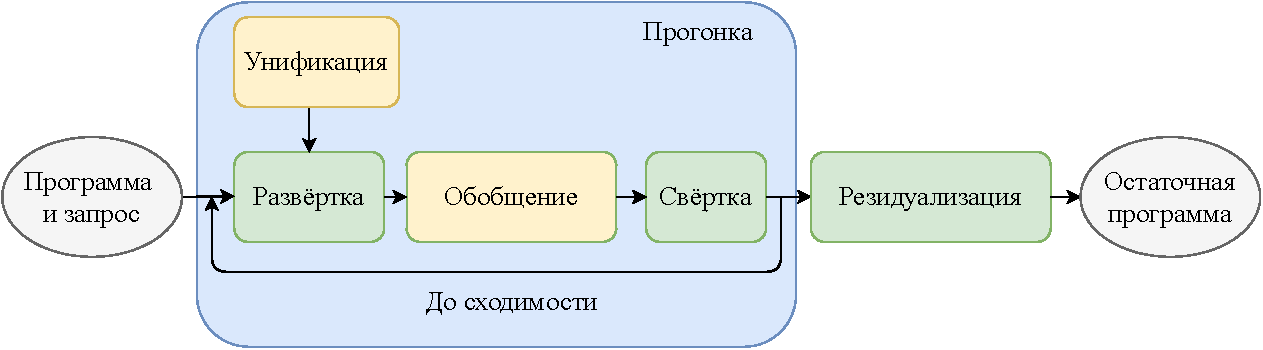
\includegraphics[width=\textwidth]{Kuklina/src/sc/scompflow.pdf}
\caption{Уточнённая схема суперкомпилятора.}
\label{fig:scompWork}
\end{figure}

Тогда необходимы модули  свёртки, развёртки, резидуализации,
а также модифицированный под задачу модуль обобщения, которые затем
нужно собрать в единый суперкомпилятор:
\begin{itemize}

\item реализация модуля свёртки заключается всего лишь в стратегии выбора множества
      конфигураций, на которые можно применять непосредственно операцию свёртки;

\item реализация модуля развёртки требует проработки стратегий символьного вычисления
      применительно для $\mu$Kanren;
\item реализация всего суперкомпилятора требует проработку структур данных, самая
      важная из которых --- граф процессов;
\item реализация резидуализации состоит из обхода графа процессов, во время
      которого происходит построение остаточной программы.
\end{itemize}

%%%%%%%%%%%%%%%%%%%%%%%%%%%%%%%%%%%%%%%%%%%%%%%%%%%%%%%%%%%%%%%%%%%
%%%%%%%%%%%%%%%%%%%%%%%%%%%%%%%%%%%%%%%%%%%%%%%%%%%%%%%%%%%%%%%%%%%
% Описание "графа" процессов
%%%%%%%%%%%%%%%%%%%%%%%%%%%%%%%%%%%%%%%%%%%%%%%%%%%%%%%%%%%%%%%%%%%
%%%%%%%%%%%%%%%%%%%%%%%%%%%%%%%%%%%%%%%%%%%%%%%%%%%%%%%%%%%%%%%%%%%
\subsubsection{Граф процессов}

Представление графа процессов в Haskell затруднено тем, что графовые
структуры данных обычно требуют ссылок на произвольные узлы,
что приводит к появлению перекрёстных ссылок. Прямая реализация этой
идеи сложна в разработке и поддержке и не является идиоматичной, хотя и используется
в реализациях суперкомпиляторов для небольших функциональных языков~\cite{scmini}.
Использование \emph{IORef}\footnote{Документация модуля Data.IORef: \url{https://hackage.haskell.org/package/base-4.11.1.0/docs/Data-IORef.html}, дата последнего посещения: 14.05.2020},
хотя и предоставляет изменяемность, приводит к неоправданному усложнению кода всего
проекта, лишая код функциональной чистоты. Также есть возможность использовать
структуру данных отображения для представления графа процессов, как это сделано
в реализации на Haskell работы~\cite{simplesc}, однако в данной работе используется
метод, который обычно применяется в частичной дедукции.

Заметим, что история вычислений представляется в виде графа из наличия
\emph{обратных рёбер}
--- то есть рёбра от детей к их родителям, --- которые появляются при свёртке,
когда ребёнок является переименованием родителя.
Тогда, если уметь сохранять или восстанавливать информацию об этой связи, то
достаточно будет представить граф в качестве \emph{дерева} процессов.
Древовидная структура однозначно отображается на процесс символьных вычислений,
а также с ними легко и идиоматично работать в Haskell.

Структура дерева процессов представлена на рисунке~\ref{fig:ptree}.

\begin{figure}[h!]
\begin{lstlisting}[mathescape,language=Haskell,extendedchars=\true,frame=single,basicstyle=\ttfamily]
type Conf = Conjunction (RelationalCall FreeVar)

type Subs = Variable $\mapsto$ Term

data Tree where
  Failure     :: Tree
  Success     :: Subst $\rarrow$ Tree
  Renaming    :: Conf $\rarrow$ Subst $\rarrow$ Tree
  Abstraction :: Conf $\rarrow$ Subst $\rarrow$ List Tree $\rarrow$ Tree
  Generalizer :: Subst $\rarrow$ Tree $\rarrow$ Tree
  Unfolding   :: Conf $\rarrow$ Subst $\rarrow$ List Tree $\rarrow$ Tree
\end{lstlisting}
\caption{Описание дерева процессов.}
\label{fig:ptree}
\end{figure}

Конфигурация \lstinline{Conf} определена как выражение со свободными переменными.
В узле дерева процессов хранится конфигурация, приведённая к форме, содержащей только конъюнкцию вызовов
реляционного отношения. Это сделано из тех соображений, что, во-первых, дизъюнкция представляет
собой ветвление вычислений, посему, соответственно, представляется как ветвление в дереве процессов,
во-вторых, унификации производятся во время символьных вычислений и добавляются в подстановку,
в-третьих, так как введение свежей переменной оказывает влияние лишь на состояние, в котором производятся вычисления,
неосмысленно сохранять его в конфигурации.

Подстановка \lstinline{Subst} соответствует своему математическому определению
как отображению из переменных в термы.
Узлы дерева процессов представляют шаги суперкомпиляции и исходы вычисления выражений:
\begin{itemize}
\item \lstinline{Failure} обозначает неудавшиеся вычисления. Такой исход
      случается при появлении противоречивых подстановок;
\item \lstinline{Success}, напротив, обозначает удавшееся вычисление, которое свелось к подстановке типа \lstinline{Subst};
\item \lstinline{Renaming} обозначает узел, конфигурация которой является переименованием какого-то родительского узла.
\item \lstinline{Abstraction} обозначает узел, который может быть обобщён на одного из
      родителей. После обобщения может появиться несколько конфигураций, которые являются
      результатом применения разделения. Эти конфигурации добавляются в качестве списка
      дочерних поддеревьев в текущий узел;
\item \lstinline{Generalizer} хранит себе обобщающий унификатор, который порождается во время обобщения
      двух термов, и поддерево с обобщённой конфигурацией;
\item \lstinline{Unfolding} обозначает шаг символьного вычисления, на котором произошёл шаг вычислений
      и по рассматриваемой на этом шаге конфигурации породились новые конфигурации.
\end{itemize}

Суперкомпилятор строит дерево процессов в глубину.

\subsubsection{Раскрытие определений отношений}
%%%%%%%%%%%%%%%%%%%%%%%%%%%%%%%%%%%%%%%%%%%%%%%%%%%%%%%%%%%%%%%%%%%
%%%%%%%%%%%%%%%%%%%%%%%%%%%%%%%%%%%%%%%%%%%%%%%%%%%%%%%%%%%%%%%%%%%
% Описание шага unfolding'а
%%%%%%%%%%%%%%%%%%%%%%%%%%%%%%%%%%%%%%%%%%%%%%%%%%%%%%%%%%%%%%%%%%%
%%%%%%%%%%%%%%%%%%%%%%%%%%%%%%%%%%%%%%%%%%%%%%%%%%%%%%%%%%%%%%%%%%%
% Стратегия символьного вычисления определяется функцией \lstinline{unfold},
% что означает ``развёртывание'' по определениям вызовы реляционных отношений.

Стратегия символьного вычисления определяется на этапе развёртки:
происходит ``развёртывание'' одного или более вызовов реляционного отношения,
при котором происходит замена вызова на определение.
Развёртка по данной конфигурации $C$ порождает
множество конфигурации $\{ C_1, \dots, C_n \}$, описывающих состояния,
в которые может перейти
процесс реального исполнения программы. Классически, шаг символьного
вычисления соответствует семантике языка, который суперкомпилируется,
и для \ukanren существует сертифицированная семантика~\cite{semanticMK},
однако описание шага символьного вычисления \ukanren для суперкомпиляции
усложнено тем, что реляционные языки не исполняются привычным образом,
как, к примеру, функциональные программы. Их ``выполнение'' происходит
через \emph{поиск}, который не отображается на классический процесс суперкомпиляции.

Тогда порождение конфигурации можно рассматривать не как непосредственный
шаг символьного вычисления,
но как определение набора состояний, которые будут рассмотрены.
% но как возможное состояние, в которое может перейти программа.
Такое состояние появляется путём раскрытия тела одного или нескольких
конъюнктов конфигурации.

К примеру, рассмотрим часть программы на \ukanren на рисунке~\ref{fig:unfoldEx}, в котором
определены отношения \lstinline{f} и \lstinline{g}.
\begin{figure}[h!]
\begin{lstlisting}
f(a) = f'(a)$\lor$f''(a)
g(a, b) = g'(a)$\land$g''(b)
\end{lstlisting}
\caption{Пример отношений для демонстрации шага символьных вычислений}
\label{fig:unfoldEx}
\end{figure}

Допустим, на шаге суперкомпиляции алгоритм обрабатывает конфигурацию
\lstinline{f($\text{v}_\text{1}$)$\land$g($\text{v}_\text{1}$, $\text{v}_\text{2}$)}
и нужно сделать шаг символьного вычисления. Рассмотрим несколько способов породить новые конфигурации.
\begin{itemize}
\item Если раскроется определение \lstinline{f}, то будут получены новые конфигурации
      \lstinline{f'($\text{v}_\text{1}$)$\land$g($\text{v}_\text{1}$, $\text{v}_\text{2}$)} и
      \lstinline{f''($\text{v}_\text{1}$)$\land$g($\text{v}_\text{1}$, $\text{v}_\text{2}$)}.
\item Если раскроется определение \lstinline{g}, то будет получена новая конфигурация
      \lstinline{f($\text{v}_\text{1}$)$\land$g'($\text{v}_\text{1}$)$\land$g''($\text{v}_\text{2}$)}.
\item Если раскроются оба определения \lstinline{f} и \lstinline{g}, то будут получены новые конфигурации
      \lstinline{f'($\text{v}_\text{1}$)$\land$g($\text{v}_\text{1}$)$\land$g''($\text{v}_\text{2}$)} и
      \lstinline{f''($\text{v}_\text{1}$)$\land$g($\text{v}_\text{1}$)$\land$g''($\text{v}_\text{2}$)}.
\end{itemize}

Последний набор конфигураций --- это полный набор состояний, в которые процесс вычислений может
прийти. В первых двух наборах, можно отметить, порождённые конфигурации не исключают
возможные состояния процессов, отображённые в последнем наборе. Они могут появиться на последующих шагах вычисления,
если перед этим ветвь исполнения не будет остановлена из-за противоречивой подстановки.

Таким образом, какой бы способ развёртывания определений ни был бы выбран, он не будет
исключать состояния, в которые процесс вычисления теоретически может прийти, но выбор
разных стратегий развёртывания может систематически приводить к разным деревьям процессов,
а следовательно --- к различным эффектам специализации.

Базовой стратегией порождения новых конфигураций выбрана \emph{полная стратегия развёртывания},
пример которой был представлен выше, при которой заменяются определения всех реляционных вызовов
конфигурации.


\subsubsection{Построение остаточной программы}

Выявление остаточной программы по дереву процессов --- \emph{резидуализация} ---
породит новые определения отношений. Больше одного отношения из дерева процессов может
появиться в случае, когда узлы \lstinline{Renaming} указывают на узлы, отличные от корня.
Поэтому первой фазой происходит пометка узлов, задающих таким образом отношения,
а также удаление поддеревьев, у которых все ветви вычисления пришли к неудаче.

Далее происходит обход дерева, во время которого генерируются узлы синтаксического дерева программы
в зависимости от типа текущего узла дерева процессов:
\begin{itemize}
\item Узел \lstinline{Unfoldable} приводит к появлению дизъюнкций подпрограмм, которые задают дети этого узла.
      Это обусловлено тем, что при прогонке в этом узле происходит ветвление вычислений;
\item Узел \lstinline{Abstraction}  приводит к появлению конъюнкций подпрограмм, которые задают дети этого узла.
	  Это обусловлено тем, что хотя операция обобщения выявляет подконъюнкции из конфигурации и рассматривает их отдельно,
	  оба поддерева, задающиеся этими подконъюнкциями, должны выполнятся в одно и то же время;
\item Узел \lstinline{Generalizer} задаёт обобщающий унификатор, который должен быть добавлен
      перед своим поддеревом;
\item Узел \lstinline{Renaming} формирует вызов реляционного отношения;
\item Узел \lstinline{Success} представляет собой успешное вычисление, предоставляющее непротиворечивую подстановку.
\end{itemize}


% В суперкомпиляции, в отличие от методов частичной дедукции, в обобщение включён
% шаг обобщения вверх, при котором происходит не подвешивание обобщённой конфигурации
% в качестве потомка конфигурации, которая обобщалась, но замена самого родителя на
% новую конфигурацию, поддерево же родителя уничтожается. Для определения
% необходимости обобщать вверх введём предикат $e_1 \genup e_2$, который
% определяет, что $e_1 \strictinst e_2$ и $e_2 \not\strictinst e_1$.
% Такое ограничение необходимо из-за того, что суперкомпилятор оперирует
% конъюнкциями выражений и делает операции разделения и обобщения вниз
% за один шаг с конъюнкциями возможно разной длины, однако для обобщения
% вверх необходимо удоставериться, что одни \todo{todo}


%%%%%%%%%%%%%%%%%%%%%%%%%%%%%%%%%%%%%%%%%%%%%%%%%%%%%%%%%%%%%%%%%%%
%%%%%%%%%%%%%%%%%%%%%%%%%%%%%%%%%%%%%%%%%%%%%%%%%%%%%%%%%%%%%%%%%%%
% Описание конкретного алгоритма суперкомпиляции
%%%%%%%%%%%%%%%%%%%%%%%%%%%%%%%%%%%%%%%%%%%%%%%%%%%%%%%%%%%%%%%%%%%
%%%%%%%%%%%%%%%%%%%%%%%%%%%%%%%%%%%%%%%%%%%%%%%%%%%%%%%%%%%%%%%%%%%
% \subsubsection{Конкретный алгоритм суперкомпиляции}

% Наличие операции обобщения вверх предполагает, что необходимо умение передвигаться по дереву вверх и изменять его.
% Реализация в Haskell этой идеи --- задача крайне нетривиальная. Возможно представлять
% деревья в мутабельных массивах, однако при обобщении необходимо удалять целые поддеревья,
% что при таком подходе сложная операция.

% Классическим способом решения этой проблемы являются \emph{зипперы}\cite{zipper}.
% Эта идиома предлагает рассматривать структуру данных как пару из элемента,
% на котором установлен фокус, и контекста, который представляется как структура данных
% с ``дыркой'', в котором сфокусированный элемент должен находиться.

% К примеру, зиппер для списка \lstinline{[1, 2, 3, 4]} при фокусе на 3 представляется
% таким образом: \lstinline{(3, ([2, 1, 0], [4, 5, 6]))}.
% Тогда перефокусировка вправо или влево на один элемент происходит за константу,
% как и замена элемента, для которой достаточно заменить первую компоненту пары.
% В то время как, в силу того, что операция взятия элемента в связном списке по индексу
% происходит за линейное время от длины списка, взятие элемента слева от 3 также
% будет происходить за линейное время, как и, соответственно, модификация списка.

% Для деревьев с произвольным количеством детей зиппер может выглядеть
% как пара из текущего узла и списка родителей, отсортированного в порядке
% близости к узлу (рисунок~\ref{fig:zipper}).
% \begin{figure}[h!]
% \begin{lstlisting}[mathescape,language=Haskell,extendedchars=\true,frame=single,basicstyle=\ttfamily]
% data Parent = Parent { children :: ListZipper Node }
% type TreeZipper = (Node, List Parent)
% \end{lstlisting}
% \caption{Пример структуры зиппера для деревьев}
% \label{fig:zipper}
% \end{figure}

% Родительский (структура \lstinline{Parent}) cписок детей представлен в виде зиппера (поле \lstinline{children})
% для списка, в котором происходит фокус: у непосредственного родителя --- на элемент в фокусе, а у остальных
% родителей --- на предыдущего в порядке сортировки.\todo{more?}

% При представлении дерева процессов в идиоме зипперов основа алгоритма суперкомпиляции
% принимает форму описания действий при смене состояния зиппера.
% \todo{TODO}

% \subsubsection{Модификации базового алгоритма суперкомпиляции}

% \textbf{Поиск узлов для переименования среди всех вычисленных поддеревьев}

% В базовом алгоритме суперкомпиляции поиск узлов на которые происходят переименования происходит
% среди родителей. Это напрямую соотносится с понятием символьных вычислений: по достижении
% узла, которое является переименованием уже встреченного, вычисление переходит на родительский узел.
% Однако довольно части встречается, что в разных поддеревьях дерева процессов стречаются одинаковые
% конфигурации, поддеревья которых оказываются полностью идентичными. В таком случае, кажется
% очевидной оптмизация, при которой мы запоминаем вычисленные поддеревья и в случае,
% когда мы встречаем схожу конфигурацию, не вычисляем поддерево заново, добавляя ссылку на него.
% \todo{Вопрос на засыпку меня же: может ли быть такое, что конфигурации являются вариантами друг друга,
% но накопленные подстановки приведут к появлению различных поддеревьев?}\\

% %%%%%%%%%%%%%%%%%%%%%%%%%%%%%%%%%%%%%%%%%%%%%%%%%%%%%%%%%%%%%%%%%%%%%%%%%%%%%%
% %%%%%%%%%%%%%%%%%%%%%%%%%%%%%%%%%%%%%%%%%%%%%%%%%%%%%%%%%%%%%%%%%%%%%%%%%%%%%%
% %%%%%%%%%%%%%%%%%%%%%%%%%%%%%%%%%%%%%%%%%%%%%%%%%%%%%%%%%%%%%%%%%%%%%%%%%%%%%%
% %%%%%%%%%%%%%%%%%%%%%%%%%%%%%%%%%%%%%%%%%%%%%%%%%%%%%%%%%%%%%%%%%%%%%%%%%%%%%%

% \textbf{Обобщение на все вычисленные узлы, не только на родительские}

% \todo{Понять, почему это не противоречит методам суперкомпиляции}

% Обобщение на вычисленные узлы приводит к тому, что деревья конфигураций
% быстрее сходятся, однако остаётся под вопросом, ухудшает ли этот подход
% качество специализации. \\


% %%%%%%%%%%%%%%%%%%%%%%%%%%%%%%%%%%%%%%%%%%%%%%%%%%%%%%%%%%%%%%%%%%%%%%%%%%%%%%
% %%%%%%%%%%%%%%%%%%%%%%%%%%%%%%%%%%%%%%%%%%%%%%%%%%%%%%%%%%%%%%%%%%%%%%%%%%%%%%
% %%%%%%%%%%%%%%%%%%%%%%%%%%%%%%%%%%%%%%%%%%%%%%%%%%%%%%%%%%%%%%%%%%%%%%%%%%%%%%
% %%%%%%%%%%%%%%%%%%%%%%%%%%%%%%%%%%%%%%%%%%%%%%%%%%%%%%%%%%%%%%%%%%%%%%%%%%%%%%

% \textbf{Стратегии развёртывания реляционных вызовов}\\

% Как уже говорилось, разные стратегии развёртывания реляционных вызовов могут привести к разным
% эффектам специализации. К примеру, полная стратегия развёртывания, которая была принята за базовую,
% приводит к \emph{таплингу} \origin{tupling}\cite{tupling} --- оптмизации, при которой
% множество проходов по одной структуре данных заменяется на один проход.

% % Может, показать, что оно круто всё строит?

% Основной недостаток базового подхода в том, что он для получения всех возможных состояний
% производит декартово производение тел вызовов в конъюнкциях, что приводит
% к сильному разрастанию дерева процессов и, как следствия, сильно требователен к вычислительным ресурсам.
% Вследствие чего реализация новых стратегий развёртывания производится не только в исследовательских,
% но и прикладных целях.

% Для лёгкой подмены стратегий суперкомпиляции был разработан специальный интерфейс \lstinline{Unfoldable}
% (рисунок~\ref{fig:unfoldable}).
% \begin{figure}[h!]
% \begin{lstlisting}
% class Unfoldable a where
%    initialize :: Conf $\rarrow$ a
%    get        :: a $\rarrow$ Conf
%    unfoldStep :: a $\rarrow$ Env $\rarrow$ List (Env, a)
% \end{lstlisting}
% \caption{Интерфейс для различных стратегий развёртывания.}
% \label{fig:unfoldable}
% \end{figure}

% Предоставляемые интерфейсом функции используются в алгоритме суперкомпиляции следующим образом:
% \begin{itemize}
% \item \lstinline{initialize} оборачивает конфигурацию в структуру, в которой может содержаться
%       вспомогательная информация для процесса развёртывания;
% \item \lstinline{get} позволяет получить конфигурацию для применения её к операциям, не зависящим
%       от стратегий;
% \item \lstinline{unfoldStep} непосредственно проводит шаг вычисления на основе текущей конфигурации
%       и её окружения, порождая новые конфигурации с соответствующими им состояниями.
% \end{itemize}

% В работе рассмотрен и реализован ряд стратегий, описанные ниже.

% \begin{itemize}
% \item {\bf Последовательная стратегия развёртывания}, при которой отслеживается,
%       какой вызов был раскрыт на предыдущем шаге, чтобы на текущем
%       раскрыть следующий за ним.

% \item {\bf Нерекурсивная стратегия развёртывания}, при которой в первую очередь
%       раскрывается нерекурсивный вызов в конфигурации. Нерекурсивность определяется
%       лишь тем, содержит ли определение реляционный вызов самого себя. Более сложный
%       анализ структуры функций не мог бы быть использован в силу того, что тогда
%       было бы необходимо реализовать класс алгоритмов анализа, что совершенно отдельная задача.

%       Ожидается, что при нерекурсивной стратегии развёртывания из конфигураций
%       будут как можно быстрее появляться выражения, которые могут быть сокращены
%       или вовсе удалены из-за унификации (к примеру, отношения, кодирующие
%       таблицы истинности, такие как \rel{and}) или привести к скорой свёрте.

% \item {\bf Рекурсивная стратегия развёртывания} при которой в первую очередь
%       раскрывается рекурсивный вызов в конфигурации. \todo{todo}.

% \item {\bf Стратегия развёртывания вызовов с минимальным количеством ветвлений},
%       при которой на каждом шаге вычисления будет появляться минимально возможное количество
%       конфигураций, что приведёт к минимальной ветвистости дерева.

% \item {\bf Стратегия развёртывания вызовов с максимльным количеством ветвлений},
%       при которой на каждом шаге вычисления будет появляться максимально возможное количество
%       конфигураций, что, с одной стороны, увеличит количество возможных состояний, но
%       потенциально может привести к сворачиванию или обобщению.
% \end{itemize}

% % \subparagraph{Смешанная стратегия развёртывания}
% % \todo{Ещё нужно бы проработать}

% %%%%%%%%%%%%%%%%%%%%%%%%%%%%%%%%%%%%%%%%%%%%%%%%%%%%%%%%%%%%%%%%%%%%%%%%%%%%%%
% %%%%%%%%%%%%%%%%%%%%%%%%%%%%%%%%%%%%%%%%%%%%%%%%%%%%%%%%%%%%%%%%%%%%%%%%%%%%%%
% %%%%%%%%%%%%%%%%%%%%%%%%%%%%%%%%%%%%%%%%%%%%%%%%%%%%%%%%%%%%%%%%%%%%%%%%%%%%%%
% %%%%%%%%%%%%%%%%%%%%%%%%%%%%%%%%%%%%%%%%%%%%%%%%%%%%%%%%%%%%%%%%%%%%%%%%%%%%%%

% \textbf{Реализация обобщения вверх}

% В суперкомпиляции, в отличие от методов частичной дедукции, для обобщения дополнительно может использоваться
% техника обобщения вверх, при которой происходит не подвешивание обобщённой конфигурации
% в качестве потомка конфигурации, которая обобщалась, но замена самого родителя на
% новую конфигурацию. Старое же поддерево родителя уничтожается.

% Для определения необходимости обобщать вверх введём предикат $e_1 \genup e_2$, который
% определяет, что $e_1 \strictinst e_2$ и $e_2 \not\strictinst e_1$.
% Такое ограничение необходимо из-за того, что суперкомпилятор оперирует
% конъюнкциями выражений и делает операции разделения и обобщения вниз
% за один шаг с конъюнкциями возможно разной длины, однако для обобщения
% вверх необходимо удостовериться, что одни \todo{todo}


% \begin{figure}[h!]
% \begin{lstlisting}
%   else if $\exists$ parent: parent $\genup$ configuration
%   then
%      node $\larrow$ generalize(configuration, parent)
%      addUp(env, tree, parent, node)
% \end{lstlisting}
% \caption{Расширение алгоритма суперкомпиляции.}
% \label{fig:scalgogenExtended}
% \end{figure}

% Наличие операции обобщения вверх предполагает, что необходимо умение передвигаться по дереву вверх и изменять его.
% Реализация в Haskell этой идеи --- задача крайне нетривиальная. Возможно представлять
% деревья в мутабельных массивах, однако при обобщении необходимо удалять целые поддеревья,
% что при таком подходе сложная операция.
% Классическим способом решения этой проблемы являются \emph{зипперы}\cite{zipper}.
% Эта идиома предлагает рассматривать структуру данных как пару из элемента,
% на котором установлен фокус, и контекста, который представляется как структура данных
% с ``дыркой'', в котором сфокусированный элемент должен находиться.
% К примеру, зиппер для списка \lstinline{[1, 2, 3, 4]} при фокусе на 3 представляется
% таким образом: \lstinline{(3, ([2, 1, 0], [4, 5, 6]))}.
% Тогда перефокусировка вправо или влево на один элемент происходит за константу,
% как и замена элемента, для которой достаточно заменить первую компоненту пары.
% В то время как, в силу того, что операция взятия элемента в связном списке по индексу
% происходит за линейное время от длины списка, взятие элемента слева от 3 также
% будет происходить за линейное время, как и, соответственно, модификация списка.
% Для деревьев с произвольным количеством детей зиппер может выглядеть
% как пара из текущего узла и списка родителей, отсортированного в порядке
% близости к узлу (рисунок~\ref{fig:zipper}).

% \begin{figure}[h!]
% \begin{lstlisting}[mathescape,language=Haskell,extendedchars=\true,frame=single,basicstyle=\ttfamily]
% data Parent = Parent { children :: ListZipper Node }
% type TreeZipper = (Node, List Parent)
% \end{lstlisting}
% \caption{Пример структуры зиппера для деревьев}
% \label{fig:zipper}
% \end{figure}

% Родительский (структура \lstinline{Parent}) cписок детей представлен в виде зиппера (поле \lstinline{children})
% для списка, в котором происходит фокус: у непосредственного родителя --- на элемент в фокусе, а у остальных
% родителей --- на предыдущего в порядке сортировки.\todo{Описать методику передвижения.}

% При представлении дерева процессов в идиоме зипперов основа алгоритма суперкомпиляции
% принимает форму описания действий при смене состояния зиппера.\todo{Описать подробнее.}\\

% Обобщение вверх приводит к тому, что происходит замена целого поддерева процессов
% предка, на которого обобщается конфигурация. Иногда это может приводить к потере
% связи между аргументами, из-за чего исчезает потенциал для возможных
% потоложительных эффектов, к примеру, протягивания констант.

% К примеру, на рисунке~\ref{fig:genup} представлено дерево процессов, при котором происходит обобщение вверх.

% \begin{figure}[h!]
% \center
% \begin{tikzpicture}[->,node distance=2cm, sibling distance=5cm]

% \tikzstyle{conf}=[rectangle,draw, rounded corners=.8ex]
% \node[conf] (root) {\rel{reverse}($a$, $a$)} ;
% \node[conf] (gen) [below of = root] {Generalizer: $\{ v_1 \mapsto a, v_2 \mapsto a \}$};
% \node[conf] (node) [below of = gen] {\rel{reverse}($v_1$, $v_2$)};
% \node (rest)[below of = node] {$\cdots$};
% \path (root) edge (gen)
%       (gen) edge (node)
%       (node) edge (rest);
% \end{tikzpicture}
% \caption{Демонстрация потери информации при обобщении вверх.}
% \label{fig:genup}
% \end{figure}

% C одной стороны, теряется потенциал для генерации более оптимальной для цели \rel{reverse}($a$, $a$)
% программы, но c другой стороны рассмотрим следующие соображения.

% В данном примере процесс прогонки происходил следующим образом: некоторое время строился
% граф для конфигурации \rel{reverse}($a$, $a$), затем вывелась конфигурация \rel{reverse}($a$, $b$).
% Если бы обобщения вверх не происходило бы, то поиск ответов в результирующей программе
% малое время провёл бы в поддереве, оптимизированном под \rel{reverse}($a$, $a$), а остальное --- в обобщённом
% \rel{reverse}($a$, $b$).

% В общем случае это может происходить не только с корнем дерева, но и в каких-то его поддеревьях.
% Однако запрет на обобщение вверх в поддеревьях может сгенерировать слишком много частных случаев
% и привести к более неэффективным программам.

% Из того, что, во-первых, есть потенциал оптимизации при сохранении информации в корне дерева и,
% во-вторых, необходимо сдреживать разрастание дерева конфигураций,
% допускается рассмотрение алгоритма с обобщением вверх с запретом на обобщение к корню дерева. \\

% %%%%%%%%%%%%%%%%%%%%%%%%%%%%%%%%%%%%%%%%%%%%%%%%%%%%%%%%%%%%%%%%%%%%%%%%%%%%%%
% %%%%%%%%%%%%%%%%%%%%%%%%%%%%%%%%%%%%%%%%%%%%%%%%%%%%%%%%%%%%%%%%%%%%%%%%%%%%%%
% %%%%%%%%%%%%%%%%%%%%%%%%%%%%%%%%%%%%%%%%%%%%%%%%%%%%%%%%%%%%%%%%%%%%%%%%%%%%%%
% %%%%%%%%%%%%%%%%%%%%%%%%%%%%%%%%%%%%%%%%%%%%%%%%%%%%%%%%%%%%%%%%%%%%%%%%%%%%%%

% \textbf{Расширение языка \ukanren c помощью операции неэквивалентности}

% Множество операции в оргинальном \ukanren покрывает все нужды реляционного программирования,
% однако на ряде программа оно вычислительно допускает пути исполнения, которые не приводят
% к успеху, однако сообщить об этом не представляется возможным.

% К примеру, на рисунке~\ref{fig:lookup} изображена операция поиска значения по ключу
% в списке пар ключ-значения \rel{lookup}.

% \begin{figure}[h!]
% \begin{lstlisting}
% $\text{lookup}^o$ K L R =
%    (K', V) :: L' $\equiv$ L $\land$
%    (K' $\equiv$ K $\land$ V $\equiv$ R $\lor$ $\text{lookup}^o$ K L' R)
% \end{lstlisting}
% \caption{Отношения поиска значения по ключу.}
% \label{fig:lookup}
% \end{figure}

% В соответствии с программой список \lstinline{L} должен иметь в голове пару из ключа и значения \lstinline{(K', V)}
% и либо  этот ключ \lstinline{K'} унифицируется с искомым ключом \lstinline{K} и
% значение \lstinline{V} --- с результатом \lstinline{R},
% либо поиск происходит в хвосте списка \lstinline{L'}. Проблема этой программы в том,
% что если унификация \lstinline{(K',V)::L' $\equiv$ L} прошла успешно и был
% найден результат, то поиск всё равно продёт во вторую ветку с рекурсивным вызовом и будет
% искать значение дальше, хотя по семантике поиска ключа в списке должен вернуться лишь одно значение.
% Более того, суперкомпилятору тоже придётся учитывать и, возможно, проводить вычисления,
% которые не принесут никакой пользы.

% В miniKanren существует операция неэквивалентности $t_1 \not\equiv t_1$, вводящее
% ограничение неэквивалентности \origin{disequality contraints}\cite{mkConstr}.
% Операция неэквивалентности определяет, что два терма $t_1$ и $t_2$ никогда не должны быть равны,
% накладывая ограничения на возможные значения свободных переменных терма.

% Расширение синтаксиса \ukanren представлено на рисунке~\ref{fig:syntaxExt}.

% \begin{figure}[h!]
% \centering
% \[\begin{array}{ccll}
% \mathcal{G}   & = & \hspace{1cm} \dots & \\
%               &   & \hspace{1cm} \mathcal{T_X}\not\equiv\mathcal{T_X} \hspace{2cm} &\mbox{дезунификация} \\
% \end{array}\]
% \caption{Расширение синтаксиса \ukanren относительно указанного на рисунке~\ref{fig:syntax}.}
% \label{fig:syntaxExt}
% \end{figure}

% Исправленная версия отношения \rel{lookup} представлена на рисунке~\ref{fig:lookupExt}.

% \begin{figure}[h!]
% \begin{lstlisting}
% $\text{lookup}^o$ K L R =
%    (K', V) :: L' $\equiv$ L $\land$
%    (K' $\equiv$ K $\land$ V $\equiv$ R $\lor$
%     K' $\not\equiv$ K $\land$ $\text{lookup}^o$ K L' R)
% \end{lstlisting}
% \caption{Исправленное отношение поиска значения по ключу.}
% \label{fig:lookupExt}
% \end{figure}

% В такой реализации две по сути исключающие друг друга ветви исполнения будут исключать друг друга
% и при вычислении запросов, и при суперкомпиляции.

% Для реализации ограничения неэквивалентности вводится новая сущность под названием
% ``хранилище ограничений'' $\Omega$ \origin{constraints store}, которое используется для проверки
% нарушений неэквивалентности. Окружение расширяется хранилищем ограничений, которое затем используется
% при унификации и при добавлении новых ограничений.

% Тогда нужно ввести следующие модификации в алгоритм унификации конфигурации, который собирает все
% операции унификации в конъюнкции перед тем, как добавить её в множество допустимых конфигураций.
% \begin{itemize}
% \item При встрече операции дезунификации $t_1 \not\equiv t_2$ необходимо произвести следующие действия.
%       Применить накопленную подстановку к термам $t_1 \theta = t_1'$ и $t_2 \theta = t_2'$ и
%       унифицировать термы $t_1'$ и $t_2'$. Если получился пустой унификатор, значит, эти термы
%       равны и ограничение нарушено. В таком случае суперкомпилятор покинет эту
%       ветвь вычислений. Если же термы не унифицируются, значит, никакая подстановка
%       в дальнейшем не нарушит ограничение. Иначе необходимо запомнить унификатор в хранилище.
% \item При встрече операции унификации $t_1 \equiv t_2$ необходимо получить их унификатор.
%       Если его не существует или он пуст, то дополнительных действий производить не нужно.
% 	  Иначе нужно проверить, не нарушает ли унификатор ограничения неэквивалентности.
% \end{itemize}

% Указанное расширение было добавлено в библиотеку с реализацией сопуствующих алгоритмов.

% Выявление остаточной программы по дереву процессов --- \emph{резидуализация} ---
% породит новые опеределения отношений. Больше одного отношения из дерева процессов может
% появиться в случае, когда узлы \lstinline{Renaming} указывают на узлы, отличные от корня.
% Поэтому первой фазой происходит пометка узлов, задающих таким образом отношения,
% а также удаление поддеревьев, у которых все ветви вычисления пришли к неудаче.

% Далее происходит обход дерева, во время которого генерируются узлы синтаксического дерева программы
% в зависимости от типа текущего узла дерева процессов:
% \begin{itemize}
% \item \lstinline{Unfoldable} узел приводит к появлению дизъюнкций подпрограмм, которые задают дети этого узла.
%       Это обусловлено тем, что при прогонке в этом узле происходит ветвеление вычислений;
% \item \lstinline{Abstraction} узел приводит к появлению конъюнкций подпрограмм, которые задают дети этого узла.
% 	  Это обусловлено тем, что хотя операция обобщения выявляет подконъюнкции из конфигурации и рассматривает их отдельно,
% 	  оба поддерева, задающиеся этими подконъюнкциями, должны выполнятся в одно и то же время;
% \item \lstinline{Generalizer} задаёт обобщающий унификатор, который должен быть добавлен
%       перед своим поддеревом;
% \item \lstinline{Renaming} формирует вызов реляционного отношения;
% \item \lstinline{Success} представляет собой успешное вычисление, предоставляющее непротиворечивую подстановку.
% \end{itemize}

